% Use only LaTeX2e, calling the article.cls class and 12-point type.
\documentclass[12pt]{article}

% Users of the {thebibliography} environment or BibTeX should use the
% scicite.sty package, downloadable from *Science* at
% www.sciencemag.org/about/authors/prep/TeX_help/ .
% This package should properly format in-text
% reference calls and reference-list numbers.

\usepackage{scicite}

% Use times if you have the font installed; otherwise, comment out the
% following line.

\usepackage{times}
\usepackage[utf8x]{inputenc}
\usepackage{scicite}
\usepackage{graphicx}
\usepackage{amsmath}
\usepackage{hyperref}
\usepackage{makeidx}
\usepackage{url}
\usepackage[italian]{babel}
\usepackage[colorinlistoftodos]{todonotes}

\usepackage{times}
\usepackage{listings}


\lstset{frame=tb,
  language=Xml,
  aboveskip=3mm,
  belowskip=3mm,
  showstringspaces=false,
  columns=flexible,
  basicstyle={\small\ttfamily},
  numbers=none,
  breaklines=true,
  breakatwhitespace=true,
  tabsize=3
}

% The preamble here sets up a lot of new/revised commands and
% environments.  It's annoying, but please do *not* try to strip these
% out into a separate .sty file (which could lead to the loss of some
% information when we convert the file to other formats).  Instead, keep
% them in the preamble of your main LaTeX source file.


% The following parameters seem to provide a reasonable page setup.

\topmargin 0.0cm
\oddsidemargin 0.2cm
\textwidth 16cm 
\textheight 21cm
\footskip 1.0cm


%The next command sets up an environment for the abstract to your paper.

\newenvironment{sciabstract}{%
\begin{quote} \bf}
{\end{quote}}


% If your reference list includes text notes as well as references,
% include the following line; otherwise, comment it out.

\renewcommand\refname{References and Notes}

% The following lines set up an environment for the last note in the
% reference list, which commonly includes acknowledgments of funding,
% help, etc.  It's intended for users of BibTeX or the {thebibliography}
% environment.  Users who are hand-coding their references at the end
% using a list environment such as {enumerate} can simply add another
% item at the end, and it will be numbered automatically.

\newcounter{lastnote}
\newenvironment{scilastnote}{%
\setcounter{lastnote}{\value{enumiv}}%
\addtocounter{lastnote}{+1}%
\begin{list}%
{\arabic{lastnote}.}
{\setlength{\leftmargin}{.22in}}
{\setlength{\labelsep}{.5em}}}
{\end{list}}

\title{Elaborazione del linguaggio naturale} 

\author{Simone Scala,$^{1}$ Bartolomeo Lombardi$^{2}$\\
    \\
    \textbf{Corso di laurea magistrale in Informatica} \\
    \textbf{Università di Bologna}
    \\\\
    \normalsize{$^{1}$simone.scala3@studio.unibo.it,}\\
    \normalsize{$^{2}$bartolomeo.lombardi@studio.unibo.it}\\
}

% Include the date command, but leave its argument blank.

\date{01 Febbraio 2017}

%%%%%%%%%%%%%%%%% END OF PREAMBLE %%%%%%%%%%%%%%%%

\begin{document} 

% Double-space the manuscript.

\baselineskip 24pt

\maketitle 

\begin{sciabstract}
  Il linguaggio è un fenomeno complesso e raramente viene inteso come sia prodotto e percepito. Un primo approccio intuitivo può indurre a pensare che il linguaggio sia costituito da parole e ogni parola sia costituita da fonemi, ma questo è certamente non vero. Il linguaggio è un processo dinamico, ove le varie parti sono raramente distinguibili. In questo lavoro, mediante \textit{CMUSphinx}, toolkit open source utilizzato per creare e allenare modelli acustici, si è proposto di sviluppare un riconoscitore vocale che riuscisse ad interpretare una serie di comandi. Dopo una prima fase, costituita da: raccolta e etichettatura dei campioni audio, si è passati alla fase di apprendimento, nonché di valutazione del modello stesso. In seguito ad un attenta analisi riguardo l'accuratezza ottenuta, si è passati allo sviluppo di un applicativo mobile nativo Android, mettendo così, in pratica, il lavoro svolto.
\end{sciabstract}

\newpage
\tableofcontents
\newpage

\section{Introduzione}
    In questa sezione introduttiva cercheremo di descrivere alcuni concetti che si collocano alla base del lavoro svolto.
    
    \begin{figure}
            \centering
            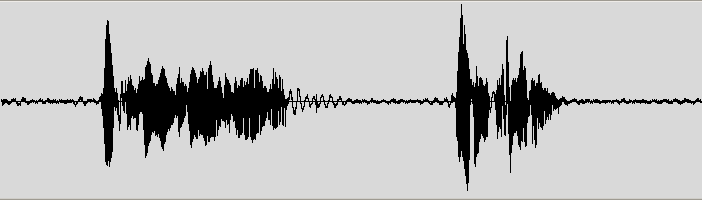
\includegraphics[scale=0.5]{waveform}
            \caption{Struttura di un waveform}
            \label{fig:first}
     \end{figure}

    \subsection{Struttura del linguaggio}
    
    Il linguaggio è un flusso d'audio continuo (fig:\ref{fig:first}) in cui gli stati piuttosto stabili si mescolano con gli stati evolutosi in modo dinamico. In questa sequenza di stati possono essere definite classi di suoni (o \textbf{foni}) più o meno equivalenti. Le proprietà acustiche di un flusso d'audio (\textbf{waveform}) corrispondente ad un fono sono spesso soggette al fenomeno della \textbf{coarticolazione}, per il quale ogni fono subisce l'influenza del contesto nel quale è articolato, vale a dire dei foni che lo precedono o lo seguono.
    L'effetto della coarticolazione può essere catturato dai \textbf{triphones}, che accorpano un singolo fono con quello immediatamente successivo e precedente. Per esempio, il fono \textit{c}  nella parola \textit{bocca} viene accorpato con il fono destro \textit{a} e con il fono sinistro \textit{c} che suona in maniera diversa rispetto allo stesso fono \textit{c} con fono destro \textit{e} e fono sinistro \textit{c} nella parola \textit{bocce}.
    L'operazione riguardante la costruzione dei triphones può risultare pesante dal punto di vista computazionale, risulta utile in tal senso individuare le parti di un triphones, anziché i triphones nel loro complesso. 
    Vengono quindi definiti detector distinti di suoni più brevi, che possano rappresentare l'intera varietà di rilevazioni acustiche. 
    Tali detector vengono chiamati \textbf{senones}.\\
    \textbf{N.B.}: un contesto potrebbe non dipendere semplicemente dal fono successivo e precedente. Piuttosto può dipendere da una funzione molto più complessa definita da un albero di decisione, o in altro modo.\\
    Un altro elemento chiave del linguaggio è rappresentato dalle \textbf{parole}, in quanto restringono in maniera significativa la dimensione dell'insieme derivante dalla combinazione dei foni. Ad esempio, se ci sono $40$ foni e una parola in media è composta da $7$ foni, possiamo avere al più $40^7$ parole, anzichè $40^{40}$.  
        
    \subsection{Processo di riconoscimento}    
    Il metodo più comunemente utilizzato nella fase di riconoscimento è il seguente:
    \begin{enumerate}
        \item viene estratto il \textit{waveform} dal flusso e viene frazionato in espressioni riconducibili alle parti stabili del grafico (silenzi)
        \item si prova poi a riconoscere cosa è stato detto in ogni espressione:
            \begin{itemize}         
                \item si calcolano tutte le possibili combinazioni tra le parole e successivamente si avvia una ricerca per trovare eventuali corrispondenze audio-parola
                \item si sceglie la corrispondenza migliore dal punto di vista probabilistico 
            \end{itemize}
    \end{enumerate}
    
    Riguardo il processo che definisce la corrispondenza audio-parola, ci sono ulteriori concetti che devono essere chiariti; il primo tra questi è il concetto di \textbf{features vector}: vettore costituito da una serie di numeri calcolati su un singolo frame, ottenuto dividendo il \textit{wavefrom} in intervalli regolari.
    Il metodo utilizzato per la generazione di tali numeri è oggetto di ricerca attiva (basata su regole), che nel caso più semplice, è derivata dallo spettro di frequenza. Il secondo, è quello di \textbf{modello}, nel quale vengono definiti oggetti matematici in grado di raccogliere gli attributi comuni della parola pronunciata. Tale modello  è chiamato \textbf{Hidden Markov Model} (HMM), il cui processo di modellazione è descritto come una sequenza di stati, che si evolvono con una certa probabilità. Lo scopo di questo modello è quello di descrivere qualsiasi processo sequenziale come un linguaggio.\\
    Riassumendo  (fig:\ref{fig:second}): l'input audio viene convertito in una sequenza di vettori di dimensione costante $Y:T = y_1,...,y_T$ nel processo chiamato \textit{feature extraction}. Dopodichè il decoder ricerca la sequenza di parole $w:L = w_1,...,w_L$, che con maggiore probabilità possa aver generato $Y$.
%    The input audio waveform from a microphone is converted into a sequence of fixed size acoustic vectors
%Y 1:T = y1,...,yT in a process called feature extraction. The decoder
%then attempts to find the sequence of words w1:L = w1,...,wL which
%is most likely to have generated Y , i.e. the decoder tries to find
%wˆ = arg max w
%{P(w|Y )}.
      \begin{figure}
            \centering
            \includegraphics[scale=0.5]{pr}
            \caption{Processo di riconoscimento}
            \label{fig:second}
     \end{figure} 
    \subsection {Definizione dei modelli}
    A seconda della struttura del linguaggio, devono essere definiti tre oggetti affinché il sistema possa effettuare correttamente il matching audio-parola:
        \begin{enumerate}
            \item Modello acustico: contiene le proprietà acustiche per ogni \textit{senone}.
            \item Dizionario della fonetica: mappa le parole con i foni; può essere definito mediante funzioni complesse, apprese con algoritmi di machine learning.
            \item Modello linguistico: usato per ottimizzare la ricerca della parola; definisce, quindi, quale parola potrebbe seguire quella precedentemente riconosciuta, riducendo così, la dimensione dell'insieme derivante dalla corrispondenza audio-parola, eliminando quelle parole che non hanno probabilità di comparire. Il modello linguistico più usato è \textbf{n-gram lenguage models} che contiene informazioni di tipo statistico riguardo la **successione delle parole.
        \end{enumerate}

    La combinazione di quest'ultimi permetterà al sistema \textbf{CMUSphinx} di decodificare l'audio ricevuto in input.
   

\newpage
\section{Tecnologie utilizzate}

    In questo paragrafo verranno descritte brevemente le principali tecnologie utilizzate durante la realizzazione del progetto.
    
    \begin{enumerate}
        \item \textbf{CMUSphinx}: toolkit open source adoperato per lo sviluppo di riconoscitori vocali. Contiene una serie di pacchetti utili all'implementazione, quelli da noi utilizzati sono i seguenti:
         \begin{itemize}         
            \item \textbf{Pocketsphinx}: libreria utilizzata per interfacciarsi con il riconoscitore implementato (scritta in C).
            \item \textbf{Sphinxbase}: libreria di supporto richiesta per \textit{Pocketsphinx}. 
            \item \textbf{Sphinxtrain}: tool utilizzato nella fase di apprendimento del modello acustico.
        \end{itemize}
        
        \item \textbf{SRI Language Modeling (Srlim)}: toolkit che offre strumenti per costruire e applicare modelli linguistici statistici (LMs). Il toolkit viene rilasciato con licenza open source, infatti può essere scaricato e usato in maniera del tutto gratuita.
        
        \item \textbf{Sequence-to-Sequence G2P}: toolkit open source, utilizzato per la conversione parola-fonema; opera attraverso reti neurali ricorrenti (RNN) con architettura \textbf{LSTM} (long short-term memory). L'implementazione, è basata su \textit{TensorFlow}, libreria software open source per l'apprendimento automatico in diversi tipi di compiti percettivi e di comprensione del linguaggio, il cui utilizzo consente un'efficiente fase di apprendimento.
        
        \item \textbf{Android}: sistema operativo per dispositivi mobili, adoperato durante lo sviluppo dell'applicativo, il quale, tramite la libreria \textit{pocketsphinx-android} appartenente al pacchetto \textit{Pocketsphinx}, ci ha permesso di testare il riconoscitore.
    
    \end{enumerate}
  
\newpage
\section{Preparazione dei dati}

    Il sistema apprende i parametri che definiscono il modello acustico attraverso una serie di campioni audio, che vengono mantenuti in un database detto \textit{training database}. Tale database, conterrà quindi le informazioni, le cui derivazioni statistiche permetteranno il funzionamento del modello acustico.\\
    La prima fase è consistita quindi, nel raccogliere tali campioni; in tal senso abbiamo registrato $30$ voci, $15$ di sesso maschile e $15$ di sesso femminile, dove ogni speaker ha pronunciato undici comandi da noi stilati. In conclusione, il nostro database di training conterrà $330$ registrazioni ($30$ voci $*$ $11$ comandi). E' stato di  fondamentale importanza, in questa fase, assicurarsi che tutte le registrazioni fossero state registrate ad una frequenza di $16$ Hz in mono stereo, così come suggerito dalla documentazione fornita da \textit{CMUSphinx}.\\       
    Ogni campione audio, contenuto nel database, è stato poi etichettato, facendo corrispondere quest'ultimo con la trascrizione della sequenza di parole contenuta nell'unità audio.
    Tale etichettatura, viene effettuata attraverso un file detto \textbf{transcript file}, nel quale le sequenze di parole sono scritte esattamente nello stesso ordine con cui compaiono nell'audio, seguite da un tag $<s>$ che associa tale sequenza (frase) con la corrispettiva registrazione.
    Riportiamo a titolo esemplificativo una parte di tale file, così come definito nel nostro modello, in cui i path dei file $wav$, contenenti le registrazioni dello speaker $anna$, sono seguiti dalle trascrizioni dei comandi (valore del tag $<s>$):
    \newpage
    \begin{lstlisting}
    <s> apri impostazioni </s> (/anna/file_1)
    <s> apri contatti </s> (/anna/file_2)
    <s> dove mi trovo </s> (/anna/file_3)
    <s> apri calcolatrice </s> (/anna/file_4)
    <s> apri calendario </s> (/anna/file_5)
    <s> componi numero </s> (/anna/file_6)
    <s> chiama tre tre uno sei tre cinque sei sei zero quattro </s> (/anna/file_7)
    <s> chiama tre tre tre due zero due sette nove otto uno </s> (/anna/file_8)
    <s> chiama tre tre tre uno zero cinque zero due otto nove </s> (/anna/file_9)
    <s> chiama zero due sette otto quattro due quattro otto otto tre </s> (/anna/file_10)    
    \end{lstlisting}
    
    Il sistema necessita poi di un dizionario, che stabilisce una corrispondenza tra la parola e le unità sonore (foni) che la compongono, in modo tale da poter derivare la sequenza di foni associati ad un segnale.
    
    \subsection{Costruzione del dizionario}    
    La maggior parte delle parole, presenti nel \textit{transcript file} sopra descritto, non erano contenute nel dizionario di Italiano, scaricabile da \textit{CMUSphinx}, ragion per cui si è ricercato un tool, che fosse in grado di mappare le parole mancanti con la sequenza fonetica corrispondente.
    A tale scopo è stato utilizzato il toolkit \textit{G2P-seq2seq}, che consente, partendo da un dizionario e un modello esistente, di apprendere regole riguardo il processo di conversione fonema-parola su parole non presenti nel dizionario di partenza.
    Per avviare il training è stato sufficiente lanciare il comando: 
    \begin{lstlisting}
g2p-seq2seq --train train-dictionary.dic --model model-folder-path
    \end{lstlisting}
    i parametri \textit{train-dictionary.dic} e \textit{model-folder-path} stanno ad indicare i dati su cui effettuare il training.
    Dopodiché, per generale la pronuncia, è stato lanciato il comando:
    \newpage
    \begin{lstlisting}
g2p-seq2seq --interactive --model model_folder_path
        
    > impostazioni
    i m p o s t a ts ts j o1 n i
    \end{lstlisting}
    data la parola in input (nell'esempio: "impostazioni"), restituisce in output, la sequenza fonetica corrispondente.
    Dopo aver iterato tale procedimento, per tutte le parole presenti nel \textit{transcript file}, abbiamo ottenuto il dizionario, che riportiamo di seguito a scopo esemplificativo.
    \begin{lstlisting}
    a a1
    a' a1
    apri a1 p r i
    calcolatrice k a1 l k o l a1 t r i tSS e
    calendario k a l e1 n d a1 r j o
    cancella k a n tSS EE l l a
    chiama k j a1 m a
    cinque tSS i1 ng k w e
    componi k o1 m p o n i
    contatti k o n t a1 t t i
    dove d o1 v e
    due d u1 e
    impostazioni i m p OO s t a ts ts j o1 n i
    mi m i1
    nove n OO v e
    numero n u1 m e r o
    otto OO t t o
    quattro k w a1 t t r o
    sei s EE i
    sette s EE t t e
    tre t r EE
    trovo t r OO v o
    uno u1 n o
    zero ts e1 r o 
    \end{lstlisting} 
    
    \subsection{Costruzione del modello linguistico}
    L'ultimo elemento richiesto dal sistema, prima di poter lanciare il training, è stato il file contenente la definizione del modello linguistico statistico, che contiene la probabilità delle combinazioni tra le parole. In un primo momento, avevamo pensato di generare un modello \textbf{unsmoothed}, dove lo stimatore di frequenza assegna probabilità uguale a $0$ a qualsiasi evento non osservato nel corpus, considerando anche la volontá di voler riconoscere comandi ben precisi. È stato poi deciso, di dare maggiore flessibilità al nostro modello, assegnando probabilità maggiore di $0$ anche agli eventi non osservati nel corpus; tali probabilità risulteranno minori rispetto a quelle degli eventi osservati, ma non uguali a $0$.\\     
    Per la generazione del modello è stato utilizzato il comando \textbf{ngram-count} di \textit{Srlim}:
    \begin{lstlisting}
ngram-count -text corpus.txt -order 2 -addsmooth 1 -lm model.lm
    \end{lstlisting} 
    che dato il corpus (lista dei comandi), l'ordine del modello (\textit{2-grams}) e data indicazione sulla tecnica di \textit{smoothing} in input, restituisce in output, il file contenente il modello linguistico (\textit{model.lm}).
    Riportiamo di seguito una parte del file generato:
    \begin{lstlisting}
\2-grams:
-0.653212	<s> apri
-1.255273	<s> cancella
-1.255273	<s> chiama
-1.255273	<s> cinque
-1.255273	<s> componi    
    \end{lstlisting} 
   la prima colonna indica che la probabilità che la frase inizi con \textit{apri} è uguale a \\ $10^{(-0.653212)} = 0.22$ e così via.
    La tecnica di smoothing utilizzata è il \textbf{Laplace Smoothing}. Questa tecnica si basa sul fatto che se abbiamo $V$ parole nel nostro vocabolario, stimeremo le probabilità del modello \textit{n-grams} come:  
    \begin{equation} 
        P_{Laplace} (w_{0}|w_{i-n+1}...w_{i-1}) = \frac{Count(w_{i-n+1}...w_{i-1}w_{i})+1}{Count(w_{i-n+1}...w_{i-1})+V} 
    \end{equation}
   
\newpage
\section{Fase di apprendimento}
Nella fase di training è stato deciso, affinchè potessimo avere un punto di confronto per il modello sviluppato ex-novo, di specializzare il modello di italiano scaricabile da \textit{CMUSphinx}, con le registrazioni dei nostri comandi.
Vedremo quindi, come è stata svolta la fase di apprendimento per entrambi i modelli.
    \subsection{Modello sviluppato}
    In seguito ad una fase di strutturazione dei file (definiti nella sezione precedente), è stato necessario apportare alcune modifiche al file di configurazione di \textit{SphinxTrain}, contenente definizioni riguardo una serie di variabili, utilizzate dal sistema durante la fase di apprendimento.
    Le variabili che hanno avuto un forte impatto sulle performance del modello sono state sostanzialmente due: il numero di \textit{senones} e il numero di \textit{densities}, definite, dopo una serie di test, come segue:
    \begin{lstlisting}
\$CFG_FINAL_NUM_DENSITIES = 8;
# Number of tied states (senones) to create in decision-tree clustering
\$CFG_N_TIED_STATES = 200;
    \end{lstlisting}
    in accordo, oltretutto, alla seguente tabella fornita dalla documentazione di \textit{CMUSphinx}:\\ \\
    \begin{tabular}{r|c|c|c|c|}
        &Vocabulary&Hours-in-db&Senones&Densities\\ \hline
        &20&5&200&8\\ \hline
        &100&10&2000&8\\ \hline
        &5000&30&4000&16\\ \hline
        &20000&80&4000&32\\ \hline
        &60000&200&6000&16\\ \hline
        &60000&2000&12000&64\\ \hline
        \end{tabular}
    \\ \\ Più \textit{senones} il modello ha, più accuratamente verrà discriminato il suono, ma d'altro canto, se si hanno troppi \textit{senones}, il modello non sarà abbastanza generico da riconoscere "unseen speech". Il resto delle variabili sono state lasciate al valore di default.\\
    Dopo esserci assicurati, che tutti gli step precedenti siano stati eseguiti correttamente, abbiamo lanciato il training eseguendo il comando:
     \begin{lstlisting}
sphinxtrain run
    \end{lstlisting}
    che restituisce in output, il modello ottenuto dall'apprendimento.
    \subsection{Modello specializzato}
    Il processo di specializzazione, date le registrazioni con relative trascrizioni (\textit{transcript file}), permette di migliorare le performance di un modello già allenato su uno specifico task. Tale processo è consigliato rispetto al training sopra descritto, quando si ha disposizione una quantità di dati limitata. Nel nostro caso, nonostante la piccola quantità di campioni audio, è risultato, come vedremo nella sezione successiva, più performante il modello costruito ex-novo.
    Il modello di partenza utilizzato è stato recuperato da \textbf{Voxforge}, database nato per raccogliere trascrizioni di dettati (speech corpus) da poter utilizzare in motori di riconoscimento vocale gratuiti e Open Source; il modello di Italiano contiene $9224$ parole e $9227$ registrazioni (circa $12$ ore).
    Per ottenere le statistiche, su i nuovi audio, è stato eseguito il comando \textit{bw} di \textit{sphinxtrain}:
    
    \begin{lstlisting}
./bw \
 -hmmdir voxforge_it_sphinx \
 -moddeffn voxforge_it_sphinx/mdef.txt \
 -ts2cbfn .cont. \
 -feat 1s_c_d_dd \
 -lda voxforge_it_sphinx/feature_transform
 -cmn current \
 -agc none \
 -dictfn voxforge_it_sphinx.dict \
 -ctlfn audio.fileids \
 -lsnfn audio.transcription \
 -accumdir .    
    \end{lstlisting} 
    i vari parametri di input sono stati recuperati dal file di configurazione del modello scaricato.
    Dopodichè, ogni parametro presente nel modello di partenza, è stato modificato eseguendo il comando \textit{map-adapt} di \textit{sphinxtrain}:
    \begin{lstlisting}
./map_adapt 
 -moddeffn voxforge_it_sphinx/mdef.txt 
 -ts2cbfn .cont. 
 -meanfn voxforge_it_sphinx/means 
 -varfn voxforge_it_sphinx/variances 
 -mixwfn voxforge_it_sphinx/mixture_weights 
 -tmatfn voxforge_it_sphinx/transition_matrices 
 -accumdir . 
 -mapmeanfn it-adapt/means 
 -mapvarfn it-adapt/variances 
 -mapmixwfn it-adapt/mixture_weights 
 -maptmatfn it-adapt/transition_matrices
    \end{lstlisting}
    
alla fine del processo il modello specializzato sarà contenuto nella cartella \textit{it-adapt}.
\newpage
\section{Risultati ottenuti}

Durante la fase di sviluppo del riconoscitore vocale, il problema più complesso è rendere la ricerca precisa (considerando quante più combinazioni possibili) e allo stesso tempo cercare di ottenere una risposta in tempi accettabili; fattori, che, possono influire in maniera significativa sulle performance del modello.
Solitamente il sistema è testato su un database di test, che possa rappresentare correttamente quello che si intende riconoscere.
Nel nostro caso, trattandosi di un task limitato, è stato sufficiente raccogliere una serie di campioni audio contenenti le registrazioni dei comandi: in tal senso sono state registrate $10$ voci, $5$ di sesso maschile e $5$ di sesso femminile, dove ogni speaker ha pronunciato undici comandi da noi stilati.\\
Nella fase di testing sono state considerate le seguenti caratteristiche (entrambe considerate in percentuale):
\begin{itemize}
    \item \textbf{Word error rate}: dato il testo originale contenente $N$ parole e dato il testo riconosciuto contenente $I$ parole inserite, $D$ parole cancellate e $S$ parole sostituite rispetto al testo originale, abbiamo che:
    \begin{equation}
        WER = \frac{I+S+D}{N}
    \end{equation}
    \item \textbf{Accuracy}: è simile al $WER$, ma non vengono contati gli inserimenti:
     \begin{equation}
        Accuracy = \frac{N-S-D}{N}
    \end{equation}
\end{itemize}
Riportiamo di seguito, a scopo esemplificativo, una parte di analisi effettuata su uno speaker inserito nel database di testing, considerando le caratteristiche sopra descritte:

 \begin{lstlisting}
ORIGINALE: chiama nove *** nove *** tre due zero due sette nove *** otto uno  
RICONOSCIUTO: chiama nove TRE nove TRE tre due zero due sette nove TRE otto uno  
Words: 11 Correct: 11 Errors: 3 Percent correct = 100.00% Error = 27.27% Accuracy = 72.73%
Insertions: 3 Deletions: 0 Substitutions: 0
  \end{lstlisting}
\textbf{N.B.}: le analisi complete riguardanti i comandi riconosciuti nella fase di testing sono reperibili nella cartella \textit{result}. 
Per lanciare il test è stato eseguito il comando \textit{pocketsphinx-batch}:

 \begin{lstlisting}
pocketsphinx_batch \
 -adcin yes \
 -cepdir wav \
 -cepext .wav \
 -ctl test.fileids \
 -lm <your.lm> \
 -dict <your.dic> \
 -hmm <your_hmm> \
 -hyp test.hyp

word_align.pl test.transcription test.hyp
  \end{lstlisting}
che dati in input i vari file definenti il modello e i path dei file audio (\textit{test.fileids}) con relative trascrizioni (\textit{test.transcription}), restituisce in output il $WER$ e l'accuratezza ottenuta. 
Tale test è stato lanciato su tre modelli: il modello sviluppato ex-novo, il modello di \textit{Voxforge} specializzato e il modello di \textit{Voxforge} senza alcuna modifica.
Riportiamo di seguito i risultati ottenuti:

\begin{lstlisting}
VOXFORGE
	
	TOTAL Words: 118 Correct: 89 Errors: 32
	TOTAL Percent correct = 75.42% Error = 27.12% Accuracy = 72.88%
	TOTAL Insertions: 3 Deletions: 12 Substitutions: 17

VOXFORGE ADOPTION

	TOTAL Words: 118 Correct: 41 Errors: 80
	TOTAL Percent correct = 34.75% Error = 67.80% Accuracy = 98.20%
	TOTAL Insertions: 3 Deletions: 35 Substitutions: 42

OUR MODEL

	TOTAL Words: 118 Correct: 118 Errors: 0
	TOTAL Percent correct = 100.00% Error = 0.00% Accuracy = 100.00%
	TOTAL Insertions: 0 Deletions: 0 Substitutions: 0
\end{lstlisting}


\section{Applicativo Android}
Dopo aver sviluppato e testato il modello si è deciso di mettere in pratica il lavoro svolto mediante un applicazione per dispositivi mobili, sviluppata per piattaforma Android tramite \textbf{Android Studio} (ambiente di sviluppo integrato (IDE) progettato specificamente per lo sviluppo di applicazioni Android).
Per importare il modello sviluppato, è stata utilizzata la libreria scaricabile da \textit{CMUSphinx}, \textit{pocketsphinx-android}, contenente una serie di metodi che permettono di rendere operativo il riconoscitore.
Non entreremo, in quanto non materia d'esame, nel dettaglio implementativo dell'applicativo, vedremo piuttosto, il metodo di ricerca utilizzato.\\
\textit{Pocketsphinx} permette di definire una lista di parole chiave su cui indirizzare la ricerca. Il vantaggio di questa ricerca è che può essere specificato un threshold per ogni parola chiave, per far si che le parole possano essere riconosciute in un discorso continuo. Tutti gli altri metodi, invece,  cercano di individuare la parola nella grammatica definita, anche nel caso in cui venga pronunciato un vocabolo non presente nella suddetta grammatica. Riportiamo di seguito la lista dei comandi, con relativo threshold, definiti per il tipo di ricerca realizzato:
\begin{lstlisting}
apri impostazioni /1e-40/
apri contatti /1e-30/
dove mi trovo /1e-45/
apri calcolatrice /1e-45/
apri calendario /1e-30/
componi numero /1e-45/
uno /1e-0.5/
due /1e-1/
tre /1e-0.5/
quattro /1e-10/
cinque /1e-10/
sei /1e-1/
sette /1e-0.1/
otto /1e-2/
nove /1e-10/
\end{lstlisting}
il valore threshold deve essere settato in maniera tale da ridurre il numero di falsi allarmi o mancati rilevamenti. Dopo una serie di test, si è giunti ai valori sopra descritti (valore definito tra $/../$).


\section{Conclusioni}
    La progettazione e la realizzazione del riconoscitore vocale non è stata esente da problemi. In primo luogo il toolkit \textit{CMUSphinx} si è prestato bene per quello che era il nostro scopo, ma le installazioni delle varie tecnologie, seppur documentate, ci hanno dato altresì problemi di compatibilità con i sistemi operativi utilizzati. In secondo luogo, nella documentazione \textit{CMUSphinx}, è stata data poca rilevanza alla configurazione dei vari parametri, necessari al sistema nella fase di apprendimento; e solo dopo un attenta analisi di soluzioni trovate sul web e una lunga fase di testing si è trovata la configurazione ottimale. La valutazione del modello ci ha dato infine risultati abbastanza soddisfacenti, anche se testati su un database di dimensioni limitate. Tali risultati hanno trovato poi un perfetto riscontro nell'applicativo android sviluppato, che sembra rispondere egregiamente ai comandi pronunciati.\\
    Naturalmente, si potrebbe pensare di estendere il corpus così da poter ottenere un riconoscitore meno specializzato di quello sviluppato, fermo restando che allo stato dell'arte i riconoscitori delle grandi compagnie, ad esempio \textbf{Google}, funzionano ormai perfettamente anche per la lingua Italiana. 
    
\clearpage\null\thispagestyle{empty}
\nocite{*} 
\bibliographystyle{plain}
\bibliography{scibib}

\end{document}